\documentclass{article}

% Language setting
% Replace `english' with e.g. `spanish' to change the document language
\usepackage[portuguese]{babel}

% Set page size and margins
% Replace `letterpaper' with `a4paper' for UK/EU standard size
\usepackage[a4paper,top=2cm,bottom=2cm,left=2cm,right=2cm,marginparwidth=1.75cm]{geometry}

% Useful packages
\usepackage{graphicx}
\usepackage{float}

\title{Relatório 2º Trabalho Prático}
\author{Bernardo Vitorino l48463, Daniel Barreiros l48452, Tomas Antunes l48511}
\date{28 de março de 2023}

\begin{document}
\maketitle

\section{Quadrado mágico como um CSP}
\subsection{Representação do problema}
\subsubsection{Estados}
A representação dos estados seguem a estrutura "e(LNT, LT)", em que LNT é a lista de variáveis não instânciadas e LT é a lista de variáveis instânciadas.

\subsubsection{Variáveis}
As variáveis são representadas na forma var((X, Y), D, V), onde X e Y são as coordenadas da varíavel, D o dominío e V o valor afetado.

\subsubsection{Restrições}
O predicado responsável por verificar as restrições é o predicado verifica\_restrições, que verifica as coordenadas, as linhas, as colunas e as diagonais, de modo a verificar que todas as coordenadas têm um valor diferente e que a soma dos valores de cada linha, coluna e diagonal é igual.

\subsubsection{Estado inicial}
O estado inicial usa a estrutura de estados do problema.

\begin{verbatim}
    estado_inicial(e([var((1,1),[1,2,3,4,5,6,7,8,9,10,11,12,13,14,15,16],_),
        var((2,1), [1,2,3,4,5,6,7,8,9,10,11,12,13,14,15, ..., 
        var((4,4), [1,2,3,4,5,6,7,8,9,10,11,12,13,14,15,16], _)],[])).
\end{verbatim}

\subsubsection{Operador sucessor}

\begin{verbatim}
    sucessor(e([var(C, D, _)| R], E), e(R, [var(C, D, CX)| E])) :- member(CX, D).
\end{verbatim}

\subsection{Resolução com o algoritmo de backtracking}
\begin{figure}[ht]
    \centering
    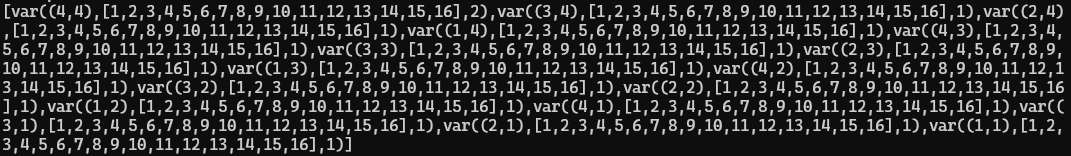
\includegraphics[width=\textwidth,height=\textheight,keepaspectratio]{image3.png}
    \caption{Output com o algoritmo backtracking}
    \label{fig:Resolução do cubo mágico com o algoritmo backtracking}
\end{figure}
\newpage
\subsection{Resolução com o algoritmo de forward checking}
\begin{figure}[ht]
    \centering
    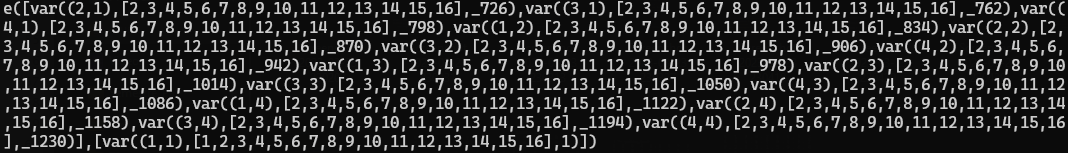
\includegraphics[width=\textwidth,height=\textheight,keepaspectratio]{image4.png}
    \caption{Output com o algoritmo forward checking}
    \label{fig:Resolução do cubo mágico com o algoritmo forward checking}
\end{figure}

\subsection{Melhoria de complexidade}
Para melhorarmos a complexidade espacial e temporal do algoritmo de pesquisa, decidimos utilizar os dois algoritmos, backtracking e forward checking, em conjunto.
\begin{figure}[h]
    \centering
    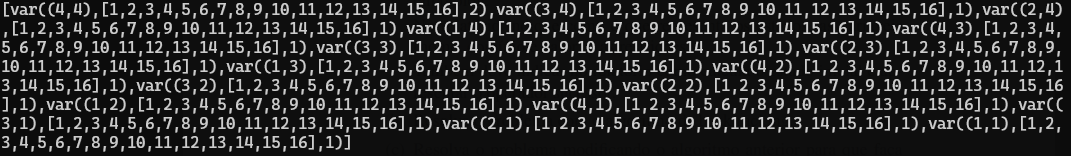
\includegraphics[width=\textwidth,height=\textheight,keepaspectratio]{image5.png}
    \caption{Output com o algoritmo backtracking e forward checking}
    \label{fig:Resolução do cubo mágico com o algoritmo backtracking e forward checking}
\end{figure}

\subsection{Exemplos}
\subsubsection{2 por 2}

\begin{figure}[ht]
    \centering
    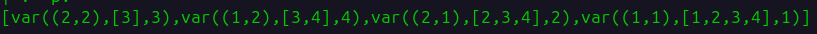
\includegraphics[width=\textwidth,height=\textheight,keepaspectratio]{image6.png}
    \caption{Resolução do cubo mágico 2 por 2 com o algoritmo forward checking e backtracking}
    \label{fig:Resolução do cubo mágico 2 por 2 com o algoritmo forward checking e backtracking}
\end{figure}
\newpage
\subsubsection{3 por 3}

\begin{figure}[ht]
    \centering
    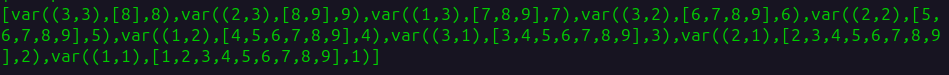
\includegraphics[width=\textwidth,height=\textheight,keepaspectratio]{image7.png}
    \caption{Resolução do cubo mágico 3 por 3 com o algoritmo forward checking e backtracking}
    \label{fig:Resolução do cubo mágico 3 por 3 com o algoritmo forward checking e backtracking}
\end{figure}

\subsubsection{4 por 4}

\begin{figure}[ht]
    \centering
    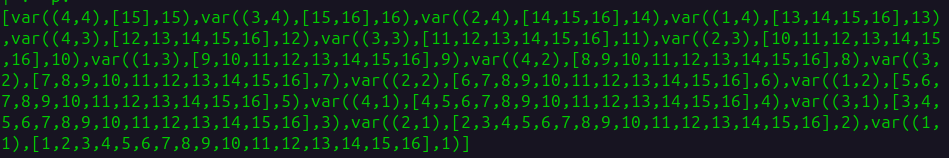
\includegraphics[width=\textwidth,height=\textheight,keepaspectratio]{image8.png}
    \caption{Resolução do cubo mágico 4 por 4 com o algoritmo forward checking e backtracking}
    \label{fig:Resolução do cubo mágico 4 por 4 com o algoritmo forward checking e backtracking}
\end{figure}


\newpage
\section{Sudoku como um CSP}
\subsection{Representação do problema}
\subsubsection{Estados}
A representação dos estados seguem a estrutura "e(LNT, LT)", em que LNT é a lista de variáveis não instânciadas e LT é a lista de variáveis instânciadas.

\subsubsection{Variáveis}
As variáveis são representadas na forma var((X, Y), D, V), onde X e Y são as coordenadas da varíavel, D o dominío e V o valor afetado.

\subsubsection{Restrições}
O predicado responsável por verificar as restrições é o predicado ve\_restrições, que verifica as linhas as colunas e os quadrantes, de modo a verificar ques todos os elementos destes três grupos são diferentes.

\subsubsection{Estado inicial}
O estado inicial usa a estrutura de estados do problema.

\begin{verbatim}
    estado_inicial(e([var((1, 1), [1,2,3,4,5,6,7,8,9], _), ..., 
        var((9, 8), [1,2,3,4,5,6,7,8,9], _), 
        var((9, 9), [1,2,3,4,5,6,7,8,9], _)],
        [var((1, 2), [1,2,3,4,5,6,7,8,9], 1), ..., 
        var((9, 3), [1,2,3,4,5,6,7,8,9], 6), 
        var((9, 6), [1,2,3,4,5,6,7,8,9], 3)])).
\end{verbatim}

\subsubsection{Operador sucessor}

\begin{verbatim}
    sucessor(e([var(N,D,_)|R],E),e(R,[var(N,D,V)|E])):- member(V,D).
\end{verbatim}

\subsection{Resolução com o algoritmo backtracking}

\begin{figure}[ht]
    \centering
    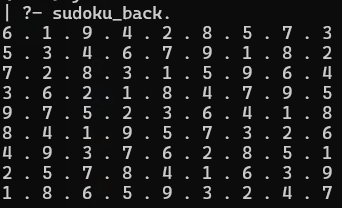
\includegraphics[width=5cm, height=4cm]{image.png}
    \caption{Output com o algoritmo backtracking}
    \label{fig:Resolução do sudoku com o algoritmo backtracking}
\end{figure}

\subsection{Resolução com o algoritmo forward checking}

\begin{figure}[ht]
    \centering
    
\includegraphics[width=15cm, height=0.37cm]{image2.png}
    \caption{Output com o algoritmo forward checking}
    \label{fig:Resolução do sudoku com o algoritmo forwward checking}
\end{figure}

Isto acontece pois é excedida a memória disponibilizada para a execução do PROLOG.


\end{document}

